\chapter{系统实现与部署}

\section{技术选型与运行依赖}

作品以 Python 实现智能体工具服务和医疗领域逻辑，
使用 FastMCP 暴露 MCP 接口，
使用两套 SQLite 数据库分别保存知识图谱和分析表。
DataMate 的数据集、文件、算子和任务状态由平台服务及 PostgreSQL 管理，
Nexent 负责智能体配置、模型调用和对话执行。
在线工作台采用轻量 HTTP 服务与 HTML、CSS、JavaScript，
关系图和统计图在浏览器中使用 SVG 绘制。

\begin{table}[H]
\centering
\caption{主要技术与用途}
\label{tab:technology-stack}
\begin{tabularx}{\textwidth}{L{3.2cm}L{4.0cm}Y}
\toprule
\textbf{技术或平台} & \textbf{对应架构层} & \textbf{项目用途} \\
\midrule
Nexent & 智能体层 &
配置三个专业智能体，绑定 MCP 工具并提供对话入口 \\
\addlinespace
DataMate & 服务层 &
管理数据集、文件、自定义算子和清洗任务 \\
\addlinespace
FastMCP & 接口层 &
注册任务一至任务三工具并返回结构化结果 \\
\addlinespace
Python & 服务层 &
实现格式处理、抽取校验、图谱事务、查询规划和成果导出 \\
\addlinespace
SQLite、PostgreSQL & 数据层 &
保存图谱事实、疾病分析表和 DataMate 平台数据 \\
\addlinespace
Docker Compose & 部署支撑 &
组织上游平台、MCP 服务、演示服务和数据卷 \\
\bottomrule
\end{tabularx}
\end{table}

\section{代码模块组织}

项目把协议入口、平台访问、业务编排、领域处理、数据存储和部署资产分开。
表~\ref{tab:module-map} 给出主要代码范围。
MCP 工具只负责参数接收、校验和结果返回，
跨步骤流程由任务服务编排，
平台调用进入客户端或适配模块，
实体、关系、分析计划等结构由领域模块统一表达。

\begin{table}[H]
\centering
\caption{主要代码范围与职责}
\label{tab:module-map}
\begin{tabularx}{\textwidth}{L{4.4cm}Y}
\toprule
\textbf{代码范围} & \textbf{职责} \\
\midrule
\repoPath{clients/} &
封装 Nexent 与 DataMate 的 HTTP 接口和身份配置 \\
\repoPath{mcp_server/tools/} &
注册智能体可调用的 MCP 工具，检查参数并整理返回结构 \\
\repoPath{mcp_server/task1/} &
数据集探查、混合格式编排、PDF 适配、状态和质量记录 \\
\repoPath{mcp_server/task2/}、\repoPath{mcp_server/kg/} &
医疗记录解析、知识抽取编排、图谱存储和分析表刷新 \\
\repoPath{core/} &
医疗抽取、九类实体校验、关系映射和图谱查询 \\
\repoPath{kg/} &
基础图谱导入、15 类关系映射和分析数据库构建 \\
\repoPath{operators/} &
DataMate 可注册的医疗数据处理与知识抽取算子 \\
\repoPath{task3/} &
统一分析服务、九类疾病事实语义层、查询计划、SQL 安全、图表策略和报告生成 \\
\repoPath{mcp_server/tools/task3_runtime.py}、\repoPath{demo/task3_interactive_demo/analysis_runtime.py} &
分别为 MCP 与 Web 入口装配同一分析服务，复用分析库路径、来源范围和大模型配置 \\
\repoPath{demo/} &
图谱浏览、数据分析和成果下载的在线工作台 \\
\repoPath{deploy/}、\repoPath{scripts/} &
环境检查、组件安装、平台注册、服务启动和验收 \\
\bottomrule
\end{tabularx}
\end{table}

\section{平台接入与智能体发布}

DataMate 接入分为数据集访问和算子运行两部分。
客户端通过平台接口解析数据集名称与标识、上传文件、读取文件清单，
并登记最终交付数据集；
任务服务创建算子实例与清洗任务，轮询任务状态并取得目标数据集。
文件内容通过 DataMate 的文件记录和数据卷读取，
数据集、任务和产物仍由平台统一管理。
医疗术语整理、表格列清理、JSON 字段清理和知识抽取算子
以算子代码和描述文件的形式注册到 DataMate，供任务调用。
任务一在线流程直接创建 DataMate 清洗任务；
任务二在线建图入口调用共享抽取服务，算子接口与该服务共用抽取模型和校验模块。

Nexent 接入分为 MCP 工具注册和智能体配置更新。
部署时先在 Nexent 建立三个智能体入口并配置所用模型。
发布脚本按智能体标识或名称读取当前版本，
从 MCP 工具清单中解析工具标识，
更新职责说明和工具绑定后发布新版本。
已有对话入口可以沿用原智能体标识，
工具集合和提示内容由脚本统一更新，数据集、任务和分析标识按工具返回值传递。
项目代码通过客户端和 MCP 接口连接两套上游平台，
医疗领域模块保持在独立目录中。

智能体配置包含职责提示、约束提示、工具集合和可选的少样本示例。
职责提示说明角色负责的业务范围，
约束提示规定工具调用顺序、真实标识传递、只读边界和错误反馈，
工具集合由 MCP 服务扫描结果绑定到已发布版本。
这些配置决定模型能够看到哪些工具，
但不替代服务端的参数校验和数据库安全检查。

项目中的三个概念具有不同职责。
FastMCP 是运行 MCP 服务并注册工具的服务框架；
MCP 工具是智能体可以调用的一个结构化工具入口；
DataMate 算子是平台内执行单个数据变换的处理单元。
例如，\path{run_task1_mixed_cleaning} 是 MCP 工具，
它在服务内部按格式创建 DataMate 清洗任务，
清洗任务再组合医疗术语规范、字段清理和文本质量处理等算子。

\section{系统部署架构}

运行环境包括 Nexent、DataMate 等上游服务，
以及 MediFlow MCP 服务、可视化服务和数据存储，
见图~\ref{fig:deployment}。
MCP 服务和可视化服务通过环境配置访问上游平台与数据库，
数据文件保存在独立卷或项目数据目录。

\begin{figure}[H]
\centering
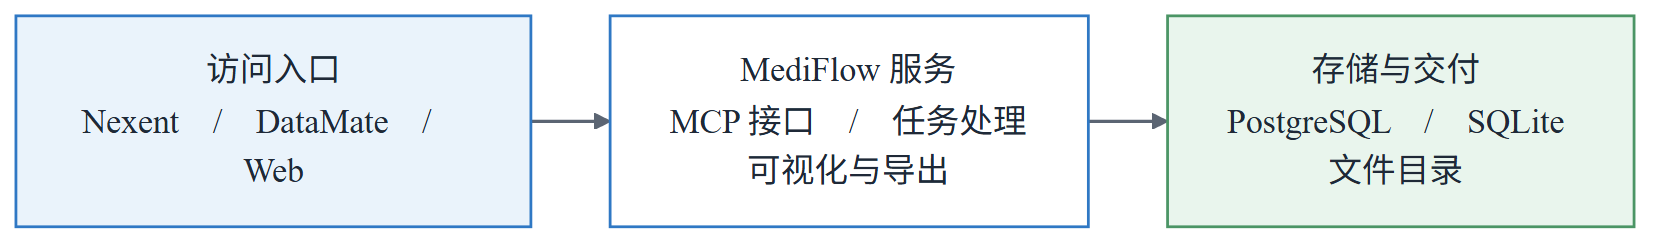
\includegraphics[width=0.90\textwidth]{figures/mermaid_deployment.png}
\caption{MediFlow 运行部署关系}
\label{fig:deployment}
\end{figure}

公开入口包括
\href{https://demo.mashiro.xin/}{MediFlow 工作台}、
\href{https://nexent.mashiro.xin/}{Nexent} 和
\href{https://datamate.mashiro.xin/}{DataMate}。
工作台用于查看图谱、提交分析问题并导出成果，任务三查询进入与 Nexent 相同的统一分析服务；
Nexent 提供三个专业智能体；
DataMate 用于管理数据集、算子和处理任务。

\section{项目交付资产}

当前运行实例建立在已准备好的 Nexent 与 DataMate 环境上。
仓库中的 \repoPath{deploy/} 目录按顺序保存环境检查、Python 依赖、
DataMate 算子注册、知识图谱与分析库构建、
MCP 服务启动与工具扫描、Nexent 智能体发布、
工作台启动和服务检查脚本。

部署目录同时提供分步脚本和顺序入口，
可以按组件安装，也可以按完整流程执行。
配置示例集中列出平台地址、数据库路径、模型接口和功能开关，
服务连接参数由部署环境注入。
图谱库与分析库由构建脚本生成，
MCP 服务和工作台在启动时读取同一组数据库配置。

\section{异常记录与故障定位}

\enlargethispage{2\baselineskip}
任务一把错误定位到文件下载、DataMate 子任务、PDF 解析或结果登记，
并保留已完成格式分组的结果；
任务二按记录返回解析与抽取状态，
图谱写入采用事务，分析刷新只在新增事实提交后执行；
任务三把计划、校验、查询和导出状态分别写入分析结果记录，
各单项查询结果独立保存。
对话入口和工作台读取同一结构化状态，
用户可以定位到数据集、文件、记录或查询。
